\section{Moments}

\subsection{Expectation and variance for weight matrix construction in NAC layers}

The weight matrix construction in NAC, is defined in scalar notation as: 
\begin{equation}
W_{h_\ell, h_{\ell-1}} = \tanh(\hat{W}_{h_\ell, h_{\ell-1}}) \sigma(\hat{M}_{h_\ell, h_{\ell-1}})
\end{equation}

Simplifying the notation of this, and re-expressing it using stochastic variables with uniform distributions this can be written as:
\begin{equation}
\begin{aligned}
W &\sim \tanh(\hat{W}) \sigma(\hat{M}) \\
\hat{W} &\sim ~ U[-r, r] \\
\hat{M} &\sim ~ U[-r, r] 
\end{aligned}
\end{equation}

Since $\tanh({\hat{W}})$ is an odd-function and $E[\hat{W}] = 0$, deriving the expectation $E[W]$ is trivial.
\begin{equation}
\mathrm{E}[W] = \mathrm{E}[\tanh(\hat{W})]\mathrm{E}[\sigma(\hat{M})] = 0 \cdot \mathrm{E}[\sigma(\hat{M})] = 0
\end{equation}

The variance is more complicated, however as $\hat{W}$ and $\hat{M}$ are independent, it can be simplified to:
\begin{equation}
\mathrm{Var}[W] = \mathrm{E}[\tanh(\hat{W})^2] \mathrm{E}[\sigma(\hat{M})^2] - \mathrm{E}[\tanh(\hat{W})]^2 \mathrm{E}[\sigma(\hat{M})]^2 = \mathrm{E}[\tanh(\hat{W})^2] \mathrm{E}[\sigma(\hat{M})^2]
\end{equation}

These second moments can be analyzed independently. First for $\mathrm{E}[\tanh(\hat{W})^2]$:
\begin{equation}
\begin{aligned}
\mathrm{E}[\tanh(\hat{W})^2] &= \int_{-\infty}^{\infty} \tanh(x)^2 f_{U[-r, r]}(x)\ \mathrm{d}x \\
&= \frac{1}{2r} \int_{-r}^{r} \tanh(x)^2\ \mathrm{d}x \\
&= \frac{1}{2r} \cdot 2 \cdot (r - \tanh(r)) \\
&= 1 - \frac{\tanh(r)}{r}
\end{aligned}
\end{equation}

Then for $\mathrm{E}[\tanh(\hat{M})^2]$:
\begin{equation}
\begin{aligned}
\mathrm{E}[\sigma(\hat{M})^2] &= \int_{-\infty}^{\infty} \sigma(x)^2 f_{U[-r, r]}(x)\ \mathrm{d}x \\
&= \frac{1}{2r} \int_{-r}^{r} \sigma(x)^2\ \mathrm{d}x \\
&= \frac{1}{2r} \left(r - \tanh\left(\frac{r}{2}\right)\right)
\end{aligned}
\end{equation}

Finally this gives the variance:
\begin{equation}
\mathrm{Var}[W] = \frac{1}{2r} \left(1 - \frac{\tanh(r)}{r}\right) \left(r - \tanh\left(\frac{r}{2}\right)\right)
\end{equation}

\subsection{Expectation and variance of $\mathrm{NAC}_{\bullet}$}
\subsubsection{Forward pass}
Assuming that each $z_{h_{\ell-1}}$ are independent the expectation can be simplified to:
\begin{equation}
\begin{aligned}
E[z_{h_\ell}] &= E\left[\exp\left(\sum_{h_{\ell-1}=1}^{H_{\ell-1}} W_{h_{\ell}, h_{\ell-1}} \log(|z_{h_{\ell-1}}| + \epsilon) \right)\right] \\
&= E\left[\prod_{h_{\ell-1}=1}^{H_{\ell-1}} \exp(W_{h_{\ell}, h_{\ell-1}} \log(|z_{h_{\ell-1}}| + \epsilon)) \right] \\
&= \prod_{h_{\ell-1}=1}^{H_{\ell-1}} E[\exp(W_{h_{\ell}, h_{\ell-1}} \log(|z_{h_{\ell-1}}| + \epsilon))] \\
&= E[\exp(W_{h_{\ell}, h_{\ell-1}} \log(|z_{h_{\ell-1}}| + \epsilon))]^{H_{\ell-1}} \\
&= E\left[(|z_{h_{\ell-1}}| + \epsilon)^{W_{h_{\ell}, h_{\ell-1}}}\right]^{H_{\ell-1}} \\
&= E\left[f(z_{h_{\ell-1}}, W_{h_{\ell}, h_{\ell-1}})\right]^{H_{\ell-1}}
\end{aligned}
\end{equation}

Here we define $f$ as a non-linear transformation function of two independent stocastic variables:
\begin{equation}
f(z_{h_{\ell-1}}, W_{h_{\ell}, h_{\ell-1}}) = (|z_{h_{\ell-1}}| + \epsilon)^{W_{h_{\ell}, h_{\ell-1}}}
\end{equation}

We then take the second order taylor approximation of $f$, around $(E[z_{h_{\ell-1}}], E[W_{h_{\ell}, h_{\ell-1}}])$.
\begin{equation}
\begin{aligned}
&E[f(z_{h_{\ell-1}}, W_{h_{\ell}, h_{\ell-1}})] \approx
E\Bigg[\\
&f(E[z_{h_{\ell-1}}], E[W_{h_{\ell}, h_{\ell-1}}])\\
&+ \begin{bmatrix}
z_{h_{\ell-1}} - E[z_{h_{\ell-1}}] \\ W_{h_{\ell}, h_{\ell-1}} - E[W_{h_{\ell}, h_{\ell-1}}]
\end{bmatrix}^T \begin{bmatrix}
\frac{\partial f(z_{h_{\ell-1}}, W_{h_{\ell}, h_{\ell-1}})}{\partial z_{h_{\ell-1}}} \\
\frac{\partial f(z_{h_{\ell-1}}, W_{h_{\ell}, h_{\ell-1}})}{\partial W_{h_{\ell}, h_{\ell-1}}}
\end{bmatrix} \Bigg\rvert_{
\begin{cases}
z_{h_{\ell-1}} = E[z_{h_{\ell-1}}] \\
W_{h_{\ell}, h_{\ell-1}} = E[W_{h_{\ell}, h_{\ell-1}}]
\end{cases}
} \\
&+ \frac{1}{2} \begin{bmatrix}
z_{h_{\ell-1}} - E[z_{h_{\ell-1}}] \\ W_{h_{\ell}, h_{\ell-1}} - E[W_{h_{\ell}, h_{\ell-1}}]
\end{bmatrix}^T \\
&\bullet \begin{bmatrix}
\frac{\partial^2 f(z_{h_{\ell-1}}, W_{h_{\ell}, h_{\ell-1}})}{\partial^2 z_{h_{\ell-1}}} & \frac{\partial^2 f(z_{h_{\ell-1}}, W_{h_{\ell}, h_{\ell-1}})}{\partial z_{h_{\ell-1}} \partial W_{h_{\ell}, h_{\ell-1}}} \\
\frac{\partial^2 f(z_{h_{\ell-1}}, W_{h_{\ell}, h_{\ell-1}})}{\partial z_{h_{\ell-1}} \partial W_{h_{\ell}, h_{\ell-1}}} & \frac{\partial^2 f(z_{h_{\ell-1}}, W_{h_{\ell}, h_{\ell-1}})}{\partial^2 W_{h_{\ell}, h_{\ell-1}}}
\end{bmatrix} \Bigg\rvert_{
\begin{cases}
z_{h_{\ell-1}} = E[z_{h_{\ell-1}}] \\
W_{h_{\ell}, h_{\ell-1}} = E[W_{h_{\ell}, h_{\ell-1}}]
\end{cases}
} \\
&\bullet \begin{bmatrix}
z_{h_{\ell-1}} - E[z_{h_{\ell-1}}] \\ W_{h_{\ell}, h_{\ell-1}} - E[W_{h_{\ell}, h_{\ell-1}}]
\end{bmatrix}\Bigg]
\end{aligned}
\end{equation}

Because $E[z_{h_{\ell-1}} - E[z_{h_{\ell-1}}]] = 0$, $E[W_{h_{\ell}, h_{\ell-1}} - E[W_{h_{\ell}, h_{\ell-1}}]] = 0$, and $Cov[z_{h_{\ell-1}}, W_{h_{\ell}, h_{\ell-1}}] = 0$. This similifies to:
\begin{equation}
\begin{aligned}
&E[f(z_{h_{\ell-1}}, W_{h_{\ell}, h_{\ell-1}})] \approx
f(E[z_{h_{\ell-1}}], E[W_{h_{\ell}, h_{\ell-1}}])\\
&+ \frac{1}{2} Var\begin{bmatrix}
z_{h_{\ell-1}} \\ W_{h_{\ell}, h_{\ell-1}}
\end{bmatrix}^T \begin{bmatrix}
\frac{\partial^2 f(z_{h_{\ell-1}}, W_{h_{\ell}, h_{\ell-1}})}{\partial^2 z_{h_{\ell-1}}} \\
\frac{\partial^2 f(z_{h_{\ell-1}}, W_{h_{\ell}, h_{\ell-1}})}{\partial^2 W_{h_{\ell}, h_{\ell-1}}}
\end{bmatrix} \Bigg\rvert_{
\begin{cases}
z_{h_{\ell-1}} = E[z_{h_{\ell-1}}] \\
W_{h_{\ell}, h_{\ell-1}} = E[W_{h_{\ell}, h_{\ell-1}}]
\end{cases}
}
\end{aligned}
\end{equation}

Inserting the derivatives and computing the inner products yields:
\begin{equation}
\begin{aligned}
&E[f(z_{h_{\ell-1}}, W_{h_{\ell}, h_{\ell-1}})] \approx
(|E[z_{h_{\ell-1}}]| + \epsilon)^{E[W_{h_{\ell}, h_{\ell-1}}]} \\
&+ \frac{1}{2} Var[z_{h_{\ell-1}}] (|E[z_{h_{\ell-1}}]| + \epsilon)^{E[W_{h_{\ell}, h_{\ell-1}}] - 2} E[W_{h_{\ell}, h_{\ell-1}}] (E[W_{h_{\ell}, h_{\ell-1}}] - 1) \\
&+ \frac{1}{2} Var[W_{h_{\ell}, h_{\ell-1}}] (|E[z_{h_{\ell-1}}]| + \epsilon)^{E[W_{h_{\ell}, h_{\ell-1}}]} \log(|E[z_{h_{\ell-1}}]| + \epsilon)^2 \\
&=1 + \frac{1}{2} Var[W_{h_{\ell}, h_{\ell-1}}] \log(|E[z_{h_{\ell-1}}]| + \epsilon)^2
\end{aligned}
\end{equation}

This gives the final expectation:
\begin{equation}
\begin{aligned}
E[z_{h_\ell}] &= E\left[f(z_{h_{\ell-1}}, W_{h_{\ell}, h_{\ell-1}})\right]^{H_{\ell-1}} \\
&\approx\left(1 + \frac{1}{2} Var[W_{h_{\ell}, h_{\ell-1}}] \log(|E[z_{h_{\ell-1}}]| + \epsilon)^2\right)^{H_{\ell-1}}
\end{aligned}
\end{equation}

As this expectation is of particular interrest, we evaluate the error of the approximation, where $W_{h_{\ell}, h_{\ell-1}} \sim U[-r_w,r_w]$ and $z_{h_{\ell-1}} \sim U[0, r_z]$. These distributions are what is used in the simple function task is done.  The result is seen in figure \ref{fig:nac-mul-expectation-estimate}.
\begin{figure}[h]
\centering
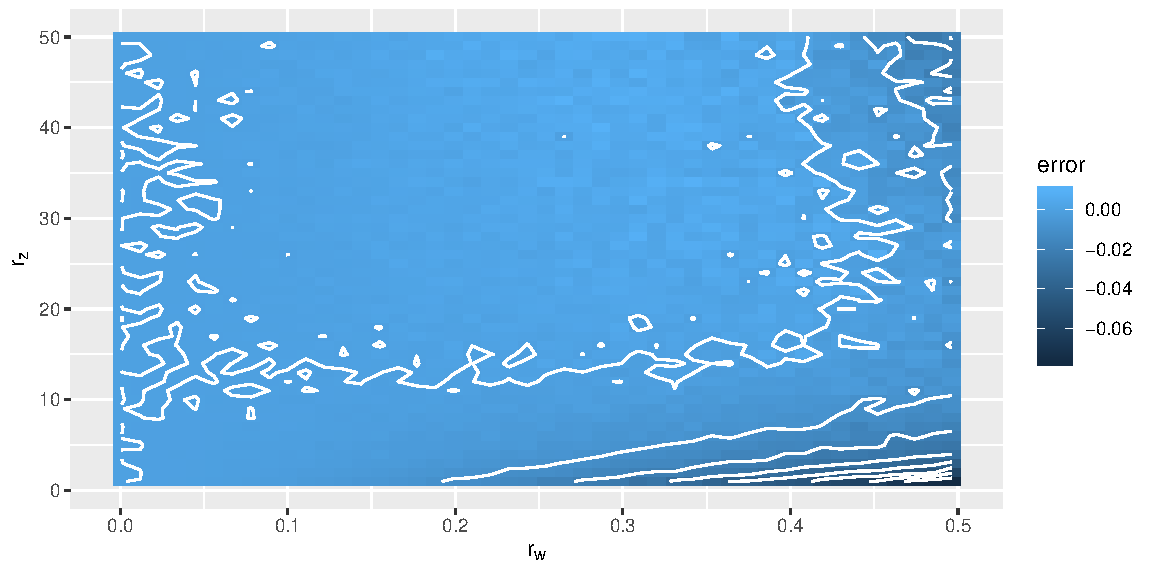
\includegraphics[width=\linewidth]{graphics/nac-mul-expectation-estimate.pdf}
\caption{Error between theoretical approximation and the numerical approximation estimated by random sampling of $100000$ observations at each combination of $r_z$ and $r_w$.}
\label{fig:nac-mul-expectation-estimate}
\end{figure}

The variance can be derived using the same assumptions about expectation and no correlation.
\begin{equation}
\begin{aligned}
Var[z_{h_\ell}] &= E[z_{h_\ell}^2] - E[z_{h_\ell}]^2 \\
&= E\left[\prod_{h_{\ell-1}=1}^{H_{\ell-1}} (|z_{h_{\ell-1}}| + \epsilon)^{2 \cdot W_{h_{\ell}, h_{\ell-1}}} \right]
- E\left[\prod_{h_{\ell-1}=1}^{H_{\ell-1}} (|z_{h_{\ell-1}}| + \epsilon)^{W_{h_{\ell}, h_{\ell-1}}}\right]^2 \\
&= E\left[f(z_{h_{\ell-1}}, 2 \cdot W_{h_{\ell}, h_{\ell-1}}) \right]^{H_{\ell-1}}
- E\left[f(z_{h_{\ell-1}}, W_{h_{\ell}, h_{\ell-1}})\right]^{2\cdot H_{\ell-1}}
\end{aligned}
\end{equation}

We already have from the expectation result that:
\begin{equation}
E\left[f(z_{h_{\ell-1}}, W_{h_{\ell}, h_{\ell-1}})\right] \approx 1 + \frac{1}{2} Var[W_{h_{\ell}, h_{\ell-1}}] \log(|E[z_{h_{\ell-1}}]| + \epsilon)^2
\end{equation}

By substitution of variable we have that:
\begin{equation}
\begin{aligned}
E\left[f(z_{h_{\ell-1}}, 2 \cdot W_{h_{\ell}, h_{\ell-1}})\right] &\approx 1 + \frac{1}{2} Var[2 \cdot W_{h_{\ell}, h_{\ell-1}}] \log(|E[z_{h_{\ell-1}}]| + \epsilon)^2 \\
&= \approx 1 + 2 \cdot Var[W_{h_{\ell}, h_{\ell-1}}] \log(|E[z_{h_{\ell-1}}]| + \epsilon)^2
\end{aligned}
\end{equation}

This gives the variance:
\begin{equation}
\begin{aligned}
Var[z_{h_\ell}] &= E\left[f(z_{h_{\ell-1}}, 2 \cdot W_{h_{\ell}, h_{\ell-1}}) \right]^{H_{\ell-1}}
- E\left[f(z_{h_{\ell-1}}, W_{h_{\ell}, h_{\ell-1}})\right]^{2\cdot H_{\ell-1}} \\
&\approx \left(1 + 2 \cdot Var[W_{h_{\ell}, h_{\ell-1}}] \log(|E[z_{h_{\ell-1}}]| + \epsilon)^2\right)^{H_{\ell-1}} \\
&- \left(1 + \frac{1}{2} \cdot Var[W_{h_{\ell}, h_{\ell-1}}] \log(|E[z_{h_{\ell-1}}]| + \epsilon)^2\right)^{2\cdot H_{\ell-1}}
\end{aligned}
\end{equation}

\subsubsection{Backward pass}

The expectation of the backpropagation term:
\begin{equation}
E[\delta_{h_\ell}] = E\left[\sum_{h_{\ell+1}=1}^{H_{\ell+1}} \delta_{h_{\ell+1}} \frac{\partial z_{h_{\ell+1}}}{\partial z_{h_\ell}}\right] = H_{\ell+1} E[\delta_{h_{\ell+1}}] E\left[\frac{\partial z_{h_{\ell+1}}}{\partial z_{h_\ell}}\right]
\end{equation}

Where we have that:
\begin{equation}
E\left[\frac{\partial z_{h_{\ell+1}}}{\partial z_{h_\ell}}\right] = E[{h_{\ell+1}}] E[W_{h_{\ell+1}, h_{\ell}}] E\left[ \frac{\mathrm{abs}'(z_{h_{\ell}})}{|z| + \epsilon}\right] = E[m_{h_{\ell+1}}] \cdot 0 \cdot E\left[ \frac{\mathrm{abs}'(z_{h_{\ell}})}{|z| + \epsilon}\right] = 0
\end{equation}

Deriving the variance is more complicated as:
\begin{equation}
\begin{aligned}
Var\left[\frac{\partial m_{h_{\ell+1}}}{\partial z_{h_\ell}}\right] &= Var\left[m_{h_{\ell+1}} W_{h_{\ell+1}, h_{\ell}} \frac{\mathrm{abs}'(z_{h_{\ell}})}{|z_{h_{\ell}}| + \epsilon}\right]
\end{aligned}
\end{equation}

Assuming independence between each term this can be simplified to as:
\begin{equation}
\begin{aligned}
Var\left[\frac{\partial z_{h_{\ell+1}}}{\partial z_{h_\ell}}\right] &= E[z_{h_{\ell+1}}^2] E[W_{h_{\ell+1}, h_{\ell}}^2] E\left[\left( \frac{\mathrm{abs}'(z_{h_{\ell}})}{|z_{h_{\ell}}| + \epsilon}\right)^2\right] \\
&- E[z_{h_{\ell+1}}]^2 E[W_{h_{\ell+1}, h_{\ell}}]^2 E\left[ \frac{\mathrm{abs}'(z_{h_{\ell}})}{|z_{h_{\ell}}| + \epsilon}\right]^2 \\
&= E[z_{h_{\ell+1}}^2] Var[W_{h_{\ell+1}, h_{\ell}}] E\left[\left( \frac{\mathrm{abs}'(z_{h_{\ell}})}{|z_{h_{\ell}}| + \epsilon}\right)^2\right] \\
&- E[z_{h_{\ell+1}}]^2 \cdot 0 \cdot E\left[ \frac{\mathrm{abs}'(z_{h_{\ell}})}{|z_{h_{\ell}}| + \epsilon}\right]^2 \\
&= E[z_{h_{\ell+1}}^2] Var[W_{h_{\ell+1}, h_{\ell}}] E\left[\left( \frac{\mathrm{abs}'(z_{h_{\ell}})}{|z_{h_{\ell}}| + \epsilon}\right)^2\right]
\end{aligned}
\end{equation}

Using Taylor approximation around $E[z_{h_{\ell}}]$ we have:
\begin{equation}
\begin{aligned}
E\left[\left(\frac{\mathrm{abs}'(z_{h_{\ell}})}{|z| + \epsilon}\right)^2\right] &\approx\frac{1}{\left(|E[z_{h_{\ell}}]| + \epsilon\right)^2} + \frac{1}{2} \frac{6}{\left(|E[z_{h_{\ell}}]| + \epsilon\right)^4} Var[z_{h_{\ell}}] \\
&= \frac{1}{\left(|E[z_{h_{\ell}}]| + \epsilon\right)^2} + \frac{3}{\left(|E[z_{h_{\ell}}]| + \epsilon\right)^4} Var[z_{h_{\ell}}]
\end{aligned}
\end{equation}

Also reusing the result for $E[z_{h_\ell}^2]$ from earlier the variance can be expressed as:
\begin{equation}
\begin{aligned}
Var\left[\frac{\partial \mathcal{L}}{\partial z_{h_{\ell-1}}}\right] &\approx Var\left[\frac{\partial \mathcal{L}}{\partial z_{h_{\ell}}}\right] H_{\ell}\ \left(1 + 2 \cdot Var[W_{h_{\ell}, h_{\ell-1}}] \log(|E[z_{h_{\ell-1}}]| + \epsilon)^2\right)^{H_{\ell-1}} \\
&\cdot Var[W_{h_{\ell}, h_{\ell-1}}] \left(\frac{1}{\left(|E[z_{h_{\ell-1}}]| + \epsilon\right)^2} + \frac{3}{\left(|E[z_{h_{\ell-1}}]| + \epsilon\right)^4} Var[z_{h_{\ell-1}}]\right)
\end{aligned}
\end{equation}

\subsection{Expectation and variance of NMU}

\subsubsection{Forward pass}

Assuming that each $z_{h_{\ell-1}}$ are independent, that $E[z_{h_{\ell-1}}] = 0$, and that $E[W_{h_{\ell-1},h_\ell}] = \nicefrac{1}{2}$ the expectation is:
\begin{equation}
\begin{aligned}
E[z_{h_\ell}] &\approx E\left[\prod_{h_{\ell-1}=1}^{H_{\ell-1}} \left(W_{h_{\ell-1},h_\ell} z_{h_{\ell-1}} + 1 - W_{h_{\ell-1},h_\ell} \right)\right] \\
&\approx E\left[W_{h_{\ell-1},h_\ell} z_{h_{\ell-1}} + 1 - W_{h_{\ell-1},h_\ell} \right]^{H_{\ell-1}} \\
&\approx \left(E[W_{h_{\ell-1},h_\ell}] E[z_{h_{\ell-1}}] + 1 - E[W_{h_{\ell-1},h_\ell}] \right)^{H_{\ell-1}} \\
&\approx\left(\frac{1}{2}\cdot0 + 1 - \frac{1}{2}\right)^{H_{\ell-1}} \\
&\approx\left(\frac{1}{2}\right)^{H_{\ell-1}}
\end{aligned}
\end{equation}

Using the same assumptions for the variance one gets:
\begin{equation}
\begin{aligned}
Var[z_{h_\ell}] &= E[z_{h_\ell}^2] - E[z_{h_\ell}]^2 \\
&\approx E[z_{h_\ell}^2] - \left(\frac{1}{2}\right)^{2 \cdot H_{\ell-1}} \\
&\approx E\left[\prod_{h_{\ell-1}=1}^{H_{\ell-1}}\left(W_{h_{\ell-1},h_\ell} z_{h_{\ell-1}} + 1 - W_{h_{\ell-1},h_\ell}\right)^2\right] - \left(\frac{1}{2}\right)^{2 \cdot H_{\ell-1}} \\
&\approx E[\left(W_{h_{\ell-1},h_\ell} z_{h_{\ell-1}} + 1 - W_{h_{\ell-1},h_\ell}\right)^2]^{H_{\ell-1}}- \left(\frac{1}{2}\right)^{2 \cdot H_{\ell-1}} \\
&\approx \Big(E[W_{h_{\ell-1},h_\ell}^2] E[z_{h_{\ell-1}}^2] - 2 E[W_{h_{\ell-1},h_\ell}^2] E[z_{h_{\ell-1}}] \\
&\quad\quad+ E[W_{h_{\ell-1},h_\ell}^2] + 2 E[W_{h_{\ell-1},h_\ell}] E[z_{h_{\ell-1}}] \\
&\quad\quad- 2 E[W_{h_{\ell-1},h_\ell}] + 1\Big)^{H_{\ell-1}}- \left(\frac{1}{2}\right)^{2 \cdot H_{\ell-1}} \\
&\approx \Big(E[W_{h_{\ell-1},h_\ell}^2] E[z_{h_{\ell-1}}^2] + E[W_{h_{\ell-1},h_\ell}^2] \\
&\quad\quad- 2 E[W_{h_{\ell-1},h_\ell}] + 1\Big)^{H_{\ell-1}}- \left(\frac{1}{2}\right)^{2 \cdot H_{\ell-1}} \\
&= \left(E[W_{h_{\ell-1},h_\ell}^2] \left(E[z_{h_{\ell-1}}^2] + 1\right)\right)^{H_{\ell-1}}- \left(\frac{1}{2}\right)^{2 \cdot H_{\ell-1}} \\
&\approx \left(\left(Var[W_{h_{\ell-1},h_\ell}] + E[W_{h_{\ell-1},h_\ell}]^2\right) \left(Var[z_{h_{\ell-1}}] + 1\right)\right)^{H_{\ell-1}}- \left(\frac{1}{2}\right)^{2 \cdot H_{\ell-1}} \\
&= \left(Var[W_{h_{\ell-1},h_\ell}] + \frac{1}{4}\right)^{H_{\ell-1}} \left(Var[z_{h_{\ell-1}}] + 1\right)^{H_{\ell-1}} - \left(\frac{1}{2}\right)^{2 \cdot H_{\ell-1}}
\end{aligned}
\end{equation}

\subsubsection{Backward pass}

For the backward pass the expectation can using the same assumptions be derived to:
\begin{equation}
\begin{aligned}
E\left[\frac{\partial \mathcal{L}}{\partial z_{h_{\ell-1}}}\right]
&= H_\ell E\left[\frac{\partial \mathcal{L}}{\partial z_{h_\ell}} \frac{\partial z_{h_\ell}}{\partial z_{h_{\ell-1}}}\right] \\
&= H_\ell E\left[\frac{\partial \mathcal{L}}{\partial z_{h_\ell}}\right] E\left[\frac{\partial z_{h_\ell}}{\partial z_{h_{\ell-1}}}\right] \\
&= H_\ell E\left[\frac{\partial \mathcal{L}}{\partial z_{h_\ell}}\right] E\left[\frac{z_{h_\ell}}{W_{h_{\ell-1},h_\ell} z_{h_{\ell-1}} + 1 - W_{h_{\ell-1},h_\ell}} W_{h_{\ell-1},h_\ell}\right] \\
&= H_\ell E\left[\frac{\partial \mathcal{L}}{\partial z_{h_\ell}}\right] E\left[\frac{z_{h_\ell}}{W_{h_{\ell-1},h_\ell} z_{h_{\ell-1}} + 1 - W_{h_{\ell-1},h_\ell}}\right]E\left[W_{h_{\ell-1},h_\ell}\right] \\
&= H_\ell E\left[\frac{\partial \mathcal{L}}{\partial z_{h_\ell}}\right] \left(\frac{1}{2}\right)^{H_{\ell-1}-1} \frac{1}{2} \\
&= E\left[\frac{\partial \mathcal{L}}{\partial z_{h_\ell}}\right] H_\ell \left(\frac{1}{2}\right)^{H_{\ell-1}} \\
&\approx 0 \cdot H_\ell \cdot \left(\frac{1}{2}\right)^{H_{\ell-1}} \\
&= 0
\end{aligned}
\end{equation}


And finally the variance for the backward pass is derived using the same assumptions.
\begin{equation}
\begin{aligned}
Var&\left[\frac{\partial \mathcal{L}}{\partial z_{h_{\ell-1}}}\right] = H_\ell Var\left[\frac{\partial \mathcal{L}}{\partial z_{h_\ell}} \frac{\partial z_{h_\ell}}{\partial z_{h_{\ell-1}}}\right] \\
&= H_\ell \Bigg(Var\left[\frac{\partial \mathcal{L}}{\partial z_{h_\ell}}\right] E\left[\frac{\partial z_{h_\ell}}{\partial z_{h_{\ell-1}}}\right]^2 + E\left[\frac{\partial \mathcal{L}}{\partial z_{h_\ell}}\right]^2 Var\left[\frac{\partial z_{h_\ell}}{\partial z_{h_{\ell-1}}}\right] \\
&+ Var\left[\frac{\partial \mathcal{L}}{\partial z_{h_\ell}}\right] Var\left[\frac{\partial z_{h_\ell}}{\partial z_{h_{\ell-1}}}\right]\Bigg) \\
&\approx Var\left[\frac{\partial \mathcal{L}}{\partial z_{h_\ell}}\right] H_\ell Var\left[\frac{\partial z_{h_\ell}}{\partial z_{h_{\ell-1}}}\right] \\
&\approx Var\left[\frac{\partial \mathcal{L}}{\partial z_{h_\ell}}\right] H_\ell \Bigg( E\left[\left(\frac{z_{h_\ell}}{W_{h_{\ell-1},h_\ell} z_{h_{\ell-1}} + 1 - W_{h_{\ell-1},h_\ell}}\right)^2\right] E[W_{h_{\ell-1},h_\ell}^2] \\
&- E\left[\frac{z_{h_\ell}}{W_{h_{\ell-1},h_\ell} z_{h_{\ell-1}} + 1 - W_{h_{\ell-1},h_\ell}}\right]^2 E[W_{h_{\ell-1},h_\ell}]^2 \Bigg) \\
&\approx Var\left[\frac{\partial \mathcal{L}}{\partial z_{h_\ell}}\right] H_\ell \Bigg( E\left[\left(\frac{z_{h_\ell}}{W_{h_{\ell-1},h_\ell} z_{h_{\ell-1}} + 1 - W_{h_{\ell-1},h_\ell}}\right)^2\right] E[W_{h_{\ell-1},h_\ell}^2] \\
&- \left(\frac{1}{2}\right)^{2 \cdot \left(H_{\ell-1}-1\right)} \left(\frac{1}{2}\right)^2\Bigg) \\
&\approx Var\left[\frac{\partial \mathcal{L}}{\partial z_{h_\ell}}\right] H_\ell \Bigg( \left(\left(Var[W_{h_{\ell-1},h_\ell}] + \frac{1}{4}\right) \left(Var[z_{h_{\ell-1}}] + 1\right)\right)^{H_{\ell-1}-1} \\
&\cdot \left(Var[W_{h_{\ell-1},h_\ell}] + \frac{1}{4}\right) - \left(\frac{1}{2}\right)^{2 \cdot H_{\ell-1}}\Bigg) \\
&= Var\left[\frac{\partial \mathcal{L}}{\partial z_{h_\ell}}\right] H_\ell \Bigg( \left(Var[W_{h_{\ell-1},h_\ell}] + \frac{1}{4}\right)^{H_{\ell-1}} \left(Var[z_{h_{\ell-1}}] + 1\right)^{H_{\ell-1}-1} \\
&- \left(\frac{1}{2}\right)^{2 \cdot H_{\ell-1}}\Bigg)
\end{aligned}
\end{equation}

\subsubsection{Initialization}

The expectation of $W_{h_{\ell-1},h_\ell}$ should be $E[W_{h_{\ell-1},h_\ell}] = \frac{1}{2}$. Using the variance approximations found, the variance should be according to the forward pass:

\begin{equation}
Var[W_{h_{\ell-1},h_\ell}] = \left((1 + Var[z_{h_\ell}])^{-H_{\ell-1}}Var[z_{h_\ell}] + (4 + 4Var[z_{h_\ell}])^{-H_{\ell-1}}\right)^{\frac{1}{H_{\ell-1}}} - \frac{1}{4}
\end{equation}

And according to the backward pass it should be:
\begin{equation}
Var[W_{h_{\ell-1},h_\ell}] = \left(H_\ell (1 + Var[z_{h_{\ell-1}}]) (4 + 4 Var[z_{h_{\ell-1}}])^{-H_{\ell-1}} + (1 + Var[z_{h_{\ell-1}}])^{1 - H_{\ell-1}}\right)^{\frac{1}{H}} - \frac{1}{4}
\end{equation}

These are both dependent on the input variance. If the input variance is know then optimal initialization is possible. However, as this is often not the case one can perhaps assume that $Var[z_{h_{\ell-1}}] = 1$. This is not an unreasonable assumption in many cases, as there may either be a normalization layer somewhere or the input is normalized. If unit variance is assumed, one gets from the forward pass:
\begin{equation}
Var[W_{h_{\ell-1},h_\ell}] = \left(2^{-H_{\ell-1}} + 8^{-H_{\ell-1}}\right)^{\frac{1}{H_{\ell-1}}} - \frac{1}{4} = \frac{1}{8} \left(\left(4^{H_{\ell-1}} + 1\right)^{H_{\ell-1}} - 2\right)
\end{equation}

And from the backward pass:
\begin{equation}
Var[W_{h_{\ell-1},h_\ell}] = \left(2 H_\ell  8^{-H_{\ell-1}} + 2^{1 - H_{\ell-1}}\right)^{\frac{1}{H}} - \frac{1}{4}
\end{equation}

The variance requirement for the backward pass is hard to satisfy, as this is dependent on two variables. However, the variance requirement from the forward pass quickly $Var[W_{h_{\ell-1},h_\ell}] = \frac{1}{4}$ may be a reasonable initialization.

